% =====================================================================
% SUPPLEMENTARY NOTE 5 — the five ablations, at length.
%
% SOURCES. Benchmark values through table1.collect(); per-epoch values and
% the decoder-reliance ratio from each arm's metrics.csv; the registered
% prediction bands and the not-ablated table from
% axw1008/docs/paper/ABLATIONS.md, written before the runs.
%
% The Results subsection states each result in one paragraph. This note
% gives the mechanism, the training record and the picture, which is where
% AW ruled the ablation detail belongs ("introduced in Results, detailed
% in Supplementary").
% =====================================================================

\section{The ablations}
\label{note:ablations}

Five single-key changes were made against the reported arm, each retrained
from scratch under the protocol of Supplementary Note~\ref{note:frontier}
and scored on the same held-out cells. The main text gives each its result;
this note gives the mechanism behind each, the training record that shows
it, the predictions registered before the runs, and the components that were
deliberately not ablated. One rule governed the wave and a test in the
repository enforces it: every arm differs from the base on exactly one
declared key. An arm that needs two keys is an arm whose question is
confounded, and one such arm was retired rather than run (below).

\subsection{Every arm beside the base}

Tables~\ref{stab:abl-bio} and~\ref{stab:abl-cost} give each arm on each
axis with its difference from the base, and Table~\ref{stab:abl-train} the
training record. Supplementary Fig.~\ref{sfig:frontier-abl} places the five
arms on the frontier's two axes with an arrow from the base to each, so the
direction of every change can be read against the six frontier arms and
the nine comparison methods. Three of the five move the model along the
same line the frontier arms trace; two move it off that line, and those two
are the ones that bear on the inductive bias.

\begin{table}[p]
\centering
\caption[Ablations, biological axes]{\textbf{The five ablations on the
biological axes, with the change against the base in parentheses.} Held-out
split, same protocol as Table~\ref{stab:arms-bio}.}
\label{stab:abl-bio}
\footnotesize\setlength{\tabcolsep}{2.5pt}
\resizebox{\textwidth}{!}{% GENERATED by figures/scripts/supp_figures.py. Do not edit by hand.
\begin{tabular}{@{}lrrrrr@{}}
\toprule
arm & cycle & family & cell type & disease & severity \\
\midrule
\elaj\,B\textsubscript{hi} (base) & 0.7346 & 0.9820 & 0.4964 & 0.3364 & 0.1157 \\
random gene grouping & 0.6780 ($-$0.0566) & 0.9606 ($-$0.0214) & 0.4889 ($-$0.0075) & 0.2698 ($-$0.0666) & 0.0572 ($-$0.0585) \\
no phase head & 0.4812 ($-$0.2534) & 0.9794 ($-$0.0026) & 0.4536 ($-$0.0428) & 0.3170 ($-$0.0194) & 0.1429 (+0.0272) \\
no ECS & 0.7397 (+0.0051) & 0.9837 (+0.0017) & 0.4994 (+0.0030) & 0.3638 (+0.0274) & 0.1232 (+0.0075) \\
no DNS sentinel & 0.7308 ($-$0.0038) & 0.9816 ($-$0.0004) & 0.4944 ($-$0.0020) & 0.3615 (+0.0251) & 0.1047 ($-$0.0110) \\
no order statistics & 0.6384 ($-$0.0962) & 0.9798 ($-$0.0022) & 0.4826 ($-$0.0138) & 0.3225 ($-$0.0139) & 0.1158 (+0.0001) \\
\bottomrule
\end{tabular}
}
\end{table}

\begin{table}[p]
\centering
\caption[Ablations, stage, grade and cost axes]{\textbf{The five ablations
on rASRM stage, grade and the two cost axes.} Donor recovery and study
separation are lower-is-better.}
\label{stab:abl-cost}
\footnotesize\setlength{\tabcolsep}{3pt}
% GENERATED by figures/scripts/supp_figures.py. Do not edit by hand.
\begin{tabular}{@{}lrrrr@{}}
\toprule
arm & stage & grade & donor & study sep. \\
\midrule
\elaj\,B\textsubscript{hi} (base) & 0.1313 & $-$0.0414 & 0.5188 & 0.7613 \\
random gene grouping & 0.1161 ($-$0.0152) & $-$0.0723 ($-$0.0309) & 0.5323 (+0.0135) & 0.7701 (+0.0088) \\
no phase head & 0.1535 (+0.0222) & $-$0.0227 (+0.0187) & 0.3754 ($-$0.1434) & 0.6523 ($-$0.1090) \\
no ECS & 0.2190 (+0.0877) & $-$0.0438 ($-$0.0024) & 0.5520 (+0.0332) & 0.8340 (+0.0727) \\
no DNS sentinel & 0.0799 ($-$0.0514) & $-$0.0549 ($-$0.0135) & 0.5207 (+0.0019) & 0.7818 (+0.0205) \\
no order statistics & 0.0918 ($-$0.0395) & $-$0.0358 (+0.0056) & 0.4943 ($-$0.0245) & 0.7600 ($-$0.0013) \\
\bottomrule
\end{tabular}

\end{table}

\begin{table}[p]
\centering
\caption[Ablations, training record]{\textbf{The training record of each
ablation.} Reconstruction loss at the selected checkpoint and at the last
epoch run; reliance is the decoder's dependence on the latent relative to
its dependence on the provenance covariates it is handed, in nats per gene,
at the selected checkpoint.}
\label{stab:abl-train}
\small
% GENERATED by figures/scripts/supp_figures.py. Do not edit by hand.
\begin{tabular}{@{}lrrrrrrr@{}}
\toprule
arm & epochs & best & train$_{nb}$ & val$_{nb}$ & train$_{nb}$ last & val$_{nb}$ last & reliance \\
\midrule
\elaj\,B\textsubscript{hi} (base) & 10 & 4 & 0.3785 & 0.4024 & 0.3762 & 0.4100 & 7.46 \\
random gene grouping & 18 & 12 & 0.3756 & 0.3911 & 0.3748 & 0.3919 & 2.43 \\
no phase head & 8 & 0 & 0.4140 & 0.4083 & 0.3772 & 0.4256 & 7.87 \\
no ECS & 10 & 4 & 0.3789 & 0.4004 & 0.3761 & 0.4146 & 8.33 \\
no DNS sentinel & 11 & 5 & 0.3777 & 0.4005 & 0.3758 & 0.4164 & 5.48 \\
no order statistics & 10 & 4 & 0.3791 & 0.3979 & 0.3760 & 0.4043 & 5.01 \\
\bottomrule
\end{tabular}

\end{table}

\begin{figure}[t]
\centering
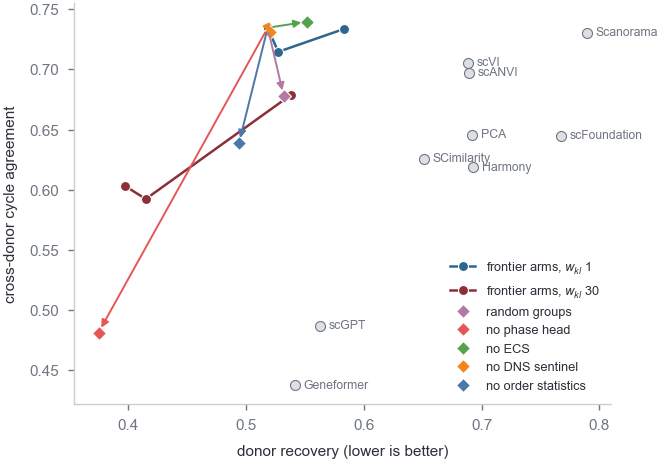
\includegraphics[width=.75\textwidth]{figures/frontier_with_ablations.png}
\caption[The ablations on the frontier]{\textbf{The five ablations on the
frontier's axes.} The six frontier arms are joined by information cost; an
arrow runs from the base to each ablation; the nine comparison methods are
grey.}
\label{sfig:frontier-abl}
\end{figure}

\subsection{Random gene grouping: the arm that fits best and holds least}

Every gene was reassigned to a random group, with group sizes, each gene's
position, parameter count, attention cost and effective gene space held
exactly as in the base. The arm trained for eighteen epochs, the longest in
the project, selected epoch 12, and reached the best held-out
reconstruction of any model including the base, 0.3911 against 0.4024
(Table~\ref{stab:abl-train}, Supplementary Fig.~\ref{sfig:loss-a}). Its
training and held-out curves descend together with the smallest and most
stable gap in the wave; a reader shown that curve alone would call it the
best-regularised model here. Every biological axis fell with it: the cycle
by 0.0566, cell family by 0.0214, disease by 0.0666 and merged severity by
0.0585, the largest biological losses of any arm on three of the four. The
decoder's reliance on the latent relative to the covariates fell from 7.46
to 2.43 (Supplementary Fig.~\ref{sfig:reliance}): with the pathway
structure gone the decoder found a cheaper route to the counts through
provenance, which is why it reconstructs better and encodes less. That is
the inductive-bias claim of the paper demonstrated rather than asserted,
and it is also why reconstruction loss is not a model-selection criterion
for a representation. Supplementary Figs.~\ref{sfig:umap-rand-family}
and~\ref{sfig:umap-rand-disease} show the latent by family and by disease
status; the family regions remain, which is consistent with cell family
being saturated across every representation in Table~1, and the disease
metric records what the picture alone cannot.

\subsection{The phase head: a third of the cycle signal, and a regulariser}

Removing the menstrual-phase head left cross-donor cycle agreement at
0.4812 against 0.7346. Both values are already chance-corrected, so the
split is their ratio: 65.5\% of the signal survives the head's removal and
the head accounts for 34.5\%. Cell family moved by 0.0026, so this is not a
broken model reporting a broken number. The training record says more than
the scalar (Supplementary Figs.~\ref{sfig:loss-a} and~\ref{sfig:traj-a}).
Without the head the held-out reconstruction loss is lowest at epoch 0,
0.4083, and rises at every epoch after, to 0.4256 at epoch 7, while the
training loss falls from 0.4140 to 0.3772; the base turns at epoch 4. The
training losses of the two arms stay within 0.0009 of each other over the
shared epochs, so the head costs nothing in fit. Checkpoint selection
therefore returned the head-free arm at epoch 0, before its structure had
arrived: its per-epoch validation cycle agreement climbs from 0.4977 at the
selected checkpoint to 0.7488 at epoch 4. Donor recovery and study
separation read 0.1203 and 0.1021 better than the base at the two selected
checkpoints and 0.0327 and 0.0010 better at epoch 7, the last both arms
ran; an under-converged latent is donor-blind because it has encoded little
of anything, and the arm's donor figure should not be quoted. What the head
does, on this record, is hold the gap between training and held-out loss
closed from the first epoch, which is a property of the whole latent rather
than of the one label it supervises. Supplementary Fig.~\ref{sfig:umap-nophase}
shows the selected checkpoint's latent by phase beside the base's
(Supplementary Fig.~\ref{sfig:umap-base-phase}).

\subsection{Elastic cell similarity: it travels the frontier}

Disabling the elastic cell similarity term moved every axis in one
direction: the cycle $+0.0051$, cell family $+0.0017$, disease $+0.0274$,
and against them donor recovery $+0.0332$ and study separation $+0.0727$
worse. A term that raises every biological axis and every cost axis when
removed is paying for mixing in biology, which makes it the same kind of
coefficient as $w_{\mathrm{kl}}$, one that moves the model along the
trade-off rather than expanding it, and its arrow in
Supplementary Fig.~\ref{sfig:frontier-abl} runs along the frontier arms'
own line. The registered prediction had assumed the term was holding cell
family together and set a band of 0.94 to 0.975 for it; family improved
instead, which is a miss worth recording because it corrected what the term
was believed to do. The embedding shows what the cost axes summarise:
Supplementary Fig.~\ref{sfig:umap-noecs} against~\ref{sfig:umap-168-1} has
single-study territories that the base does not.

\subsection{The order statistics: a cycle mechanism}

Each group's readout hands forward a learned summary token and eight
pooled order statistics of its gene tokens, 288 numbers in all; the
ablation keeps the summary token alone, 32 numbers. Parameter count is
unchanged because the statistics are computed rather than learned. The
cycle fell by 0.0962 and the sixty-way cell type by 0.0138 while cell
family moved by 0.0022 and reconstruction improved, 0.3979 against 0.4024.
The registered band for the cycle was 0.66 to 0.73 and the arm landed at
0.6384, below it, so the statistics matter more than predicted and on one
axis in particular. What a weighted average discards is the shape of a
group's distribution, and on this corpus that shape carries the cycle
rather than cell identity.

\subsection{The DNS sentinel: visible, not measurable}

Replacing the sentinel for genes a study never assayed with a zero moved
every scalar by less than 0.011 except study separation, which worsened by
0.0205, and disease, which rose by 0.0251. On the scalars this is the
smallest change in the wave. The embedding disagrees: with the phase head,
the adversary and the per-study normalisation all still running, the
latent breaks into single-study regions where the base has a continuum
(Supplementary Fig.~\ref{sfig:umap-nodns} against~\ref{sfig:umap-168-1}),
and the decoder's reliance ratio falls from 7.46 to 5.48. A neighbourhood
metric is insensitive to this kind of reorganisation, which is a limit of
the metric rather than evidence the component does nothing. The reasoning
registered for this arm was that the sentinel suppresses a study signal;
the prediction stands as written but the reasoning was revised before the
run landed, because marking unmeasured genes explicitly makes a panel more
legible rather than less. What the sentinel buys is that the model never
learns a gene is silent in a cell type when nobody looked at it, and
absence of measurement stays distinct from a measured absence.

\begin{figure}[t]
\centering
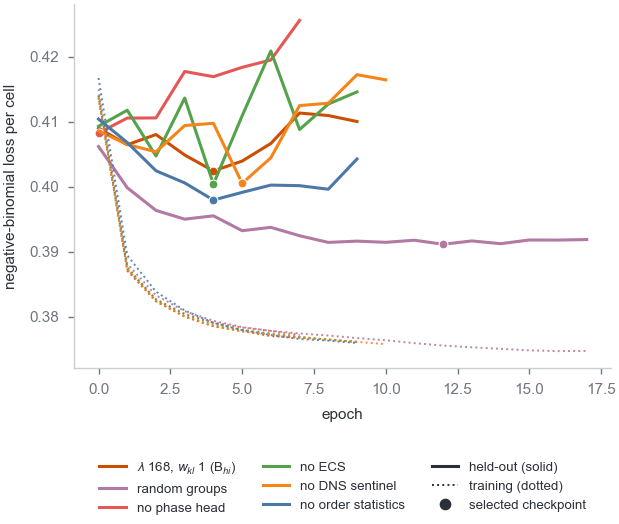
\includegraphics[width=.75\textwidth]{figures/training_loss_ablations.png}
\caption[Reconstruction loss per epoch, ablations]{\textbf{Held-out
(solid) and training (dotted) reconstruction loss per epoch for the base
and the five ablations}, with each arm's selected checkpoint marked.}
\label{sfig:loss-a}
\end{figure}

\begin{figure}[t]
\centering
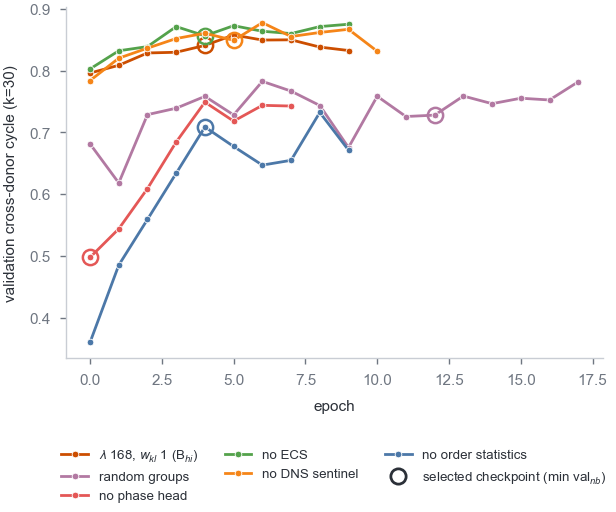
\includegraphics[width=.75\textwidth]{figures/trajectory_cycle_ablations.png}
\caption[Validation cycle agreement per epoch, ablations]{\textbf{Validation
cross-donor cycle agreement per epoch}, $k = 30$ on 19{,}972 validation
cells. The head-free arm's selected checkpoint is its first epoch; its
value four epochs later is 0.7488.}
\label{sfig:traj-a}
\end{figure}

\begin{figure}[t]
\centering
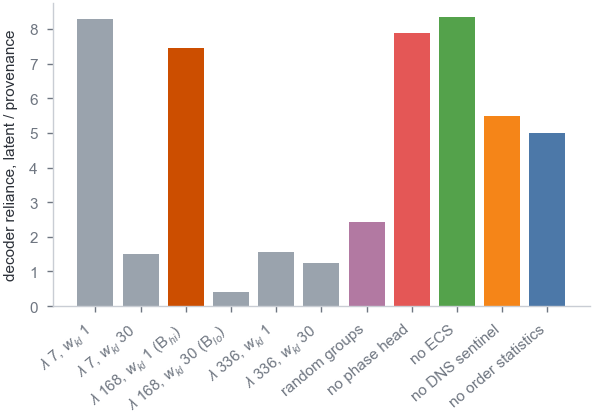
\includegraphics[width=.65\textwidth]{figures/reliance_ratio_all_arms.png}
\caption[Decoder reliance on the latent, all arms]{\textbf{The decoder's
reliance on the latent relative to the provenance covariates, every arm, at
its selected checkpoint.}}
\label{sfig:reliance}
\end{figure}

\subsection{What was predicted before the runs}

Each arm had bands registered in its configuration file before training
(Table~\ref{stab:abl-pred}). Six of eleven landed. The misses carry more
than the hits: the head-free arm's donor recovery landed under its band
because the arm was returned at epoch 0; cell family did not fall without
the similarity term or the sentinel, and rose without the former; the
cycle fell further than predicted without the order statistics. Each of
those corrected a belief about what the component was for, and the text
above is written to the outcome rather than to the prediction.

\begin{table}[t]
\centering
\caption[Registered predictions, ablations]{\textbf{The bands registered
before each ablation ran, against the outcomes.} Benchmark terms; donor
recovery is lower-is-better.}
\label{stab:abl-pred}
\small
% GENERATED by figures/scripts/supp_figures.py. Do not edit by hand.
\begin{tabular}{@{}llrrl@{}}
\toprule
arm & axis & registered band & observed &  \\
\midrule
no phase head & cycle & 0.450 to 0.620 & 0.4812 & landed \\
no phase head & family & 0.975 to 0.985 & 0.9794 & landed \\
no phase head & donor & 0.480 to 0.560 & 0.3754 & missed \\
no ECS & family & 0.940 to 0.975 & 0.9837 & missed \\
no ECS & donor & 0.480 to 0.580 & 0.5520 & landed \\
no order statistics & family & 0.955 to 0.978 & 0.9798 & missed \\
no order statistics & cycle & 0.660 to 0.730 & 0.6384 & missed \\
no DNS sentinel & donor & 0.500 to 0.580 & 0.5207 & landed \\
no DNS sentinel & family & 0.960 to 0.980 & 0.9816 & missed \\
random gene grouping & family & 0.930 to 0.970 & 0.9606 & landed \\
random gene grouping & cycle & 0.620 to 0.720 & 0.6780 & landed \\
\bottomrule
\end{tabular}

\end{table}

\subsection{What was not ablated, and why}

A reviewer will ask about each of these, so the reasons are recorded
(Table~\ref{stab:not-ablated}). One arm was built and then retired before
running: a latent with four circular dimensions in place of eight Gaussian
ones. The width would have matched the base at sixteen while the intrinsic
dimension fell to twelve, because a point on a circle has one degree of
freedom carried in two numbers, and a circle carries less than a Gaussian
coordinate besides, since it is compact and its divergence from the prior
is a function of concentration alone. Whichever way the arm came back it
could not have been attributed to geometry, so it was deleted rather than
deprioritised.

\begin{table}[t]
\centering
\caption[Components deliberately not ablated]{\textbf{Components not
ablated, and the reason each was left alone.}}
\label{stab:not-ablated}
\small
\begin{tabular}{@{}p{38mm}p{112mm}@{}}
\toprule
component & why no ablation \\
\midrule
adversarial weight $\lambda_{\mathrm{dab}}$ & the frontier grid already varies it over 7, 168 and 336 at two latent prices; a point at zero would restate what six runs show \\
decoder conditioning on study, platform and tissue & a conditional VAE conditions its decoder by definition; removing it tests the class of model rather than this one \\
domain-specific batch normalisation & no clean switch exists: freezing the per-study affine leaves per-study normalisation statistics in place, so the arm would measure something it could not name \\
one study per batch & required by the normalisation above, so it cannot move independently \\
two-stage against flat attention & flat attention at matched effective gene space is roughly 50 million parameters against 1.1 million; the claim is arithmetic rather than a run \\
bilinear decoder, library-size composition, negative binomial over Poisson & argued from parameter cost and from the measured overdispersion of the counts \\
the aggregation-stage readout & excluded from the order-statistics arm so that it stays one variable; untested at the cell stage \\
gene masking & measured a very small effect in development and is described as a detail rather than claimed \\
\bottomrule
\end{tabular}
\end{table}

\begin{figure}[p]\centering
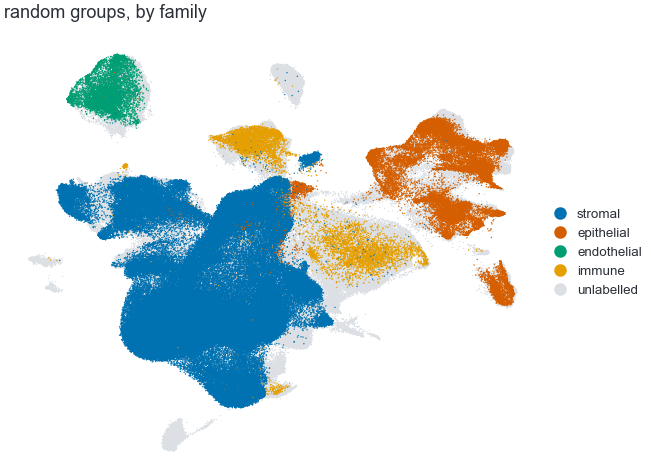
\includegraphics[width=.7\textwidth]{figures/umap_a1_randgroups_family.png}
\caption[UMAP by family, random grouping]{\textbf{The random-grouping
latent, by cell family.} Grey cells carry no annotation.}
\label{sfig:umap-rand-family}\end{figure}

\begin{figure}[p]\centering
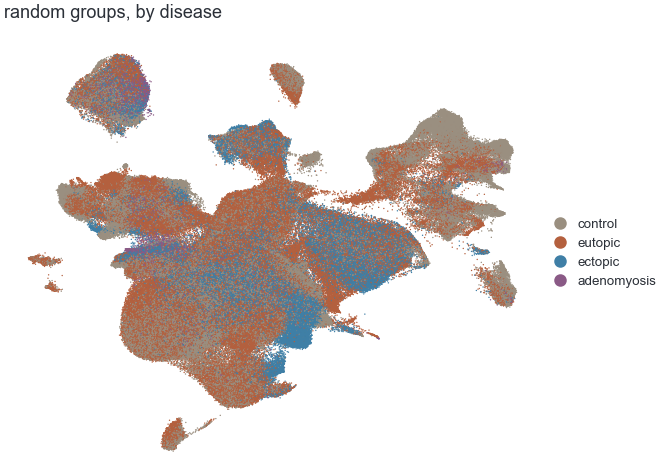
\includegraphics[width=.7\textwidth]{figures/umap_a1_randgroups_disease.png}
\caption[UMAP by disease, random grouping]{\textbf{The random-grouping
latent, by disease status}; compare Supplementary
Fig.~\ref{sfig:umap-base-disease}.}
\label{sfig:umap-rand-disease}\end{figure}

\begin{figure}[p]\centering
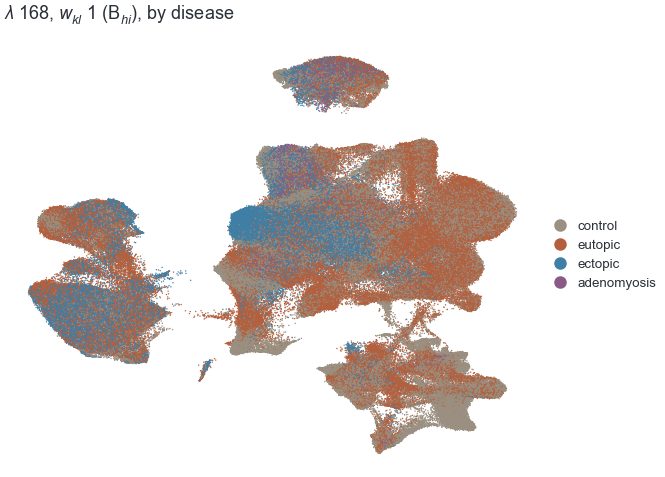
\includegraphics[width=.7\textwidth]{figures/umap_p1_dab168_kl1_disease.png}
\caption[UMAP by disease, \elaj\,B\textsubscript{hi}]{\textbf{The reported
latent, by disease status.}}
\label{sfig:umap-base-disease}\end{figure}

\begin{figure}[p]\centering
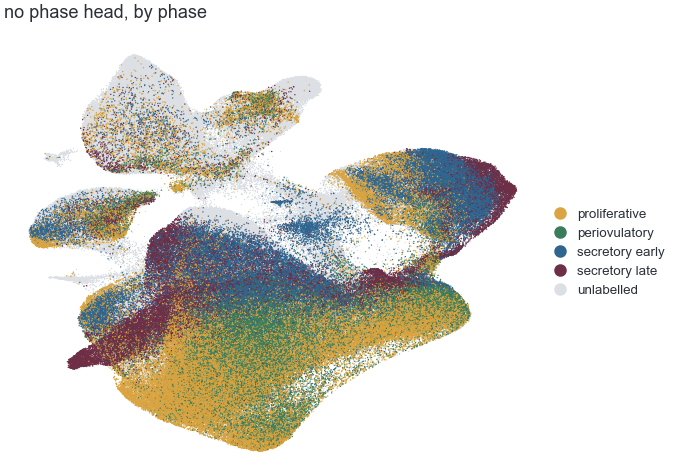
\includegraphics[width=.7\textwidth]{figures/umap_a1_nophase_phase.png}
\caption[UMAP by phase, no phase head]{\textbf{The head-free latent at
its selected checkpoint, by menstrual phase}; compare Supplementary
Fig.~\ref{sfig:umap-base-phase}.}
\label{sfig:umap-nophase}\end{figure}

\begin{figure}[p]\centering
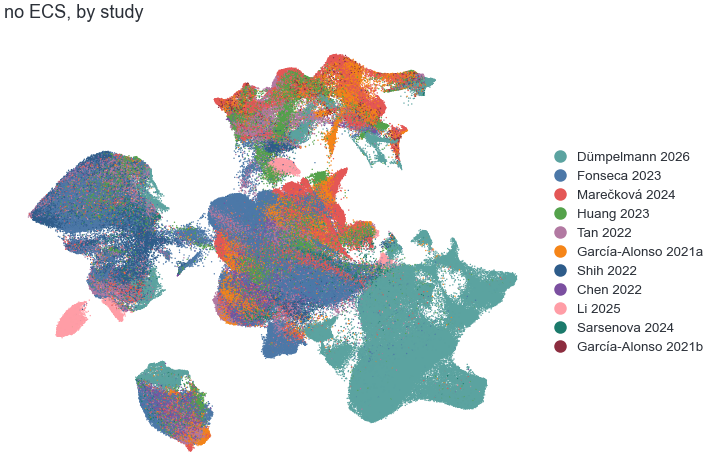
\includegraphics[width=.7\textwidth]{figures/umap_a1_noecs_study.png}
\caption[UMAP by study, no ECS]{\textbf{The latent without the elastic
cell similarity term, by study}; compare Supplementary
Fig.~\ref{sfig:umap-168-1}.}
\label{sfig:umap-noecs}\end{figure}

\begin{figure}[p]\centering
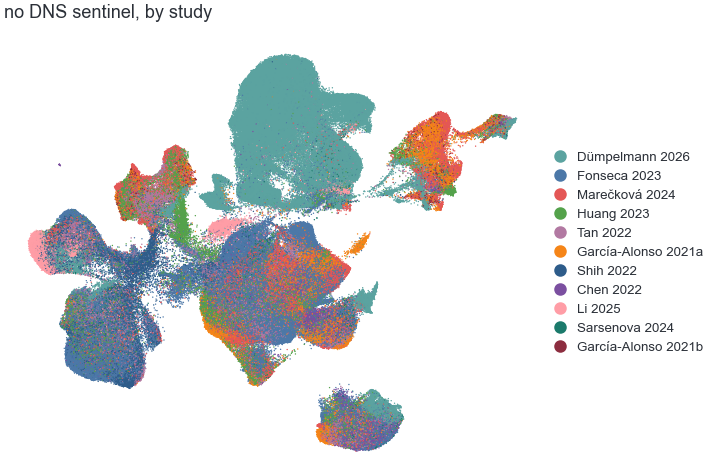
\includegraphics[width=.7\textwidth]{figures/umap_a1_nodns_study.png}
\caption[UMAP by study, no DNS sentinel]{\textbf{The latent without the
sentinel for unmeasured genes, by study}; compare Supplementary
Fig.~\ref{sfig:umap-168-1}.}
\label{sfig:umap-nodns}\end{figure}
